\section{State Patterns}

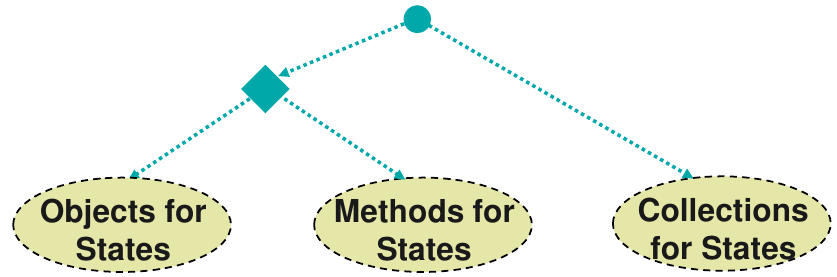
\includegraphics[width=\linewidth]{state.png}

\subsection{Objects for State}

Resultiert in vielen Klassen und Strukturen

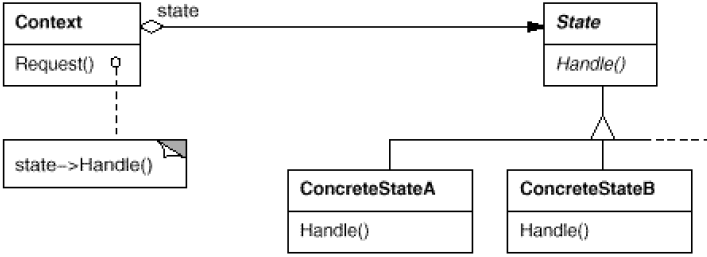
\includegraphics[width=\linewidth]{objects_for_state.png} \\

\textbf{Dynamic}

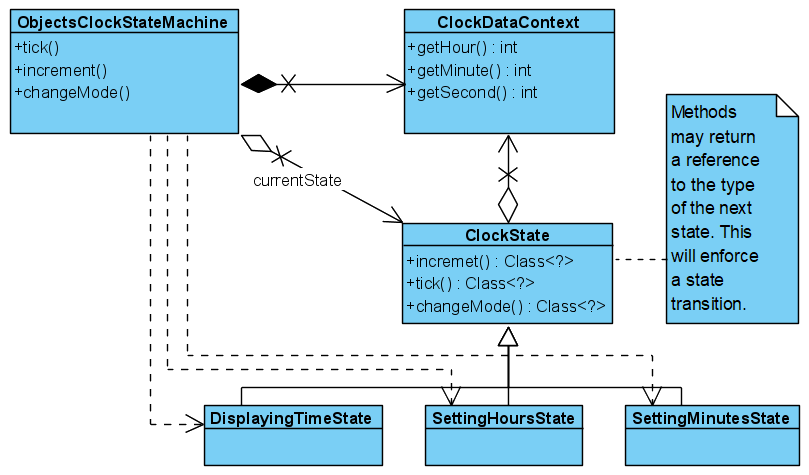
\includegraphics[width=\linewidth]{objects_for_state_dynamic.png}

\subsubsection{Problem}
\begin{itemize}
    \item Das Verhalten eines Objekts hängt von seinem Zustand ab, und es muss sein Verhalten zur Laufzeit ändern.
    \item Operationen haben grosse, mehrteilige bedingte Anweisungen (Flags), die vom Zustand abhängen
\end{itemize}
\subsubsection{Intent}
Wie kann ein Objekt entsprechend seinem Zustand ohne mehrteilige bedingte Anweisungen handeln?

\subsubsection{Solution}

Erlaubt einem Objekt das Verhalten zu ändern, wenn dessen internen Zustand sich ändert. Das Objekt scheint die Klasse zu ändern

\subsubsection{Consequences}
\textbf{Liabilities}
\begin{itemize}
    \item Das Pattern ist komplex, aber deckt die Komplexität nicht angemessen ab
    \item Das Pattern ist in vielen Fällen overkill
    \item Name suggests problem domain rather than the solution
\end{itemize}

\subsection{Methods for State}

Propagiert eine einzelne Klasse mit vielen Methoden

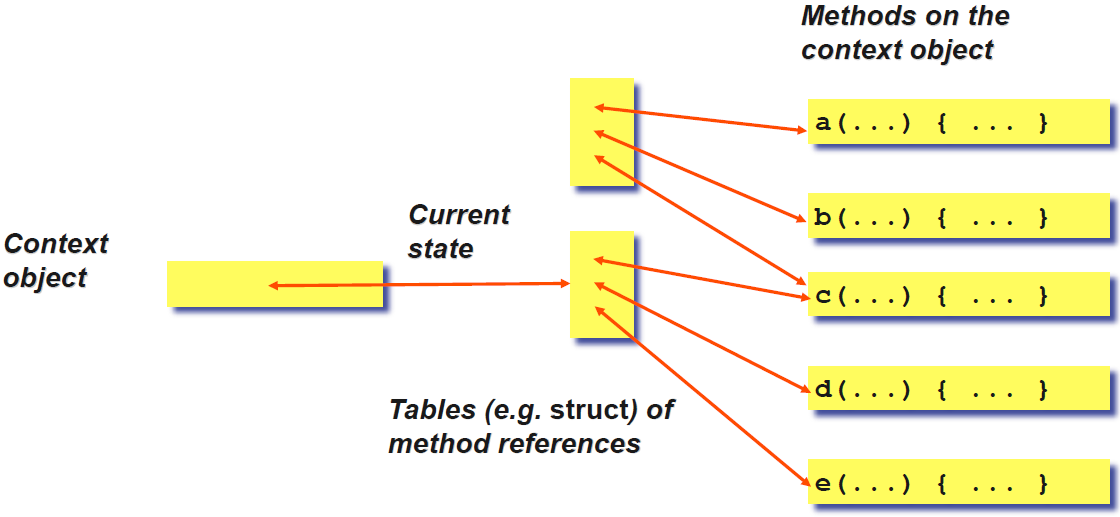
\includegraphics[width=\linewidth]{method_for_state.png} \\

\textbf{Dynamics}

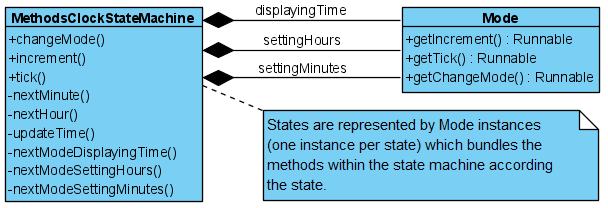
\includegraphics[width=\linewidth]{method_for_state_dynamic.png}

\subsubsection{Solution}

Jeder Zustand repräsentiert eine Tabelle oder Record von Methoden referenzen. Die Methoden-Referenzen liegen auf dem State Machine (context) Objekt

\subsubsection{Consequences}
\textbf{Benefits}
\begin{itemize}
    \item Ermöglicht es einer Klasse, all ihre verschiedenen Verhaltensweisen in gewöhnlichen Methoden auszudrücken, die sie selbst betreffen
    \item Verhalten ist an die State Machine gekoppelt, anstelle über mehrere kleine Klassen fragmentiert
    \item Jedes distinct Verhalten ist an eine eigene Methode zugewiesen
    \item Kein Objekt Kontext muss herumgereicht werden, Methoden können auf den internen Zustand der State Machine zugreifen
\end{itemize}
\vspace{10pt}
\textbf{Liabilities}
\begin{itemize}
    \item Benötigt zusätzliche 2 Levels von Umwegen um ein Methoden Aufruf aufzulösen
    \item Die State Machine kann viel länger dauern als beabsichtigt oder überschaubar ist
\end{itemize}

\subsection{Collection for State}

Ermöglicht mehrere State Machines mit der selben Logik zu managen und splittet Logik und Transaction Management in 2 Klassen

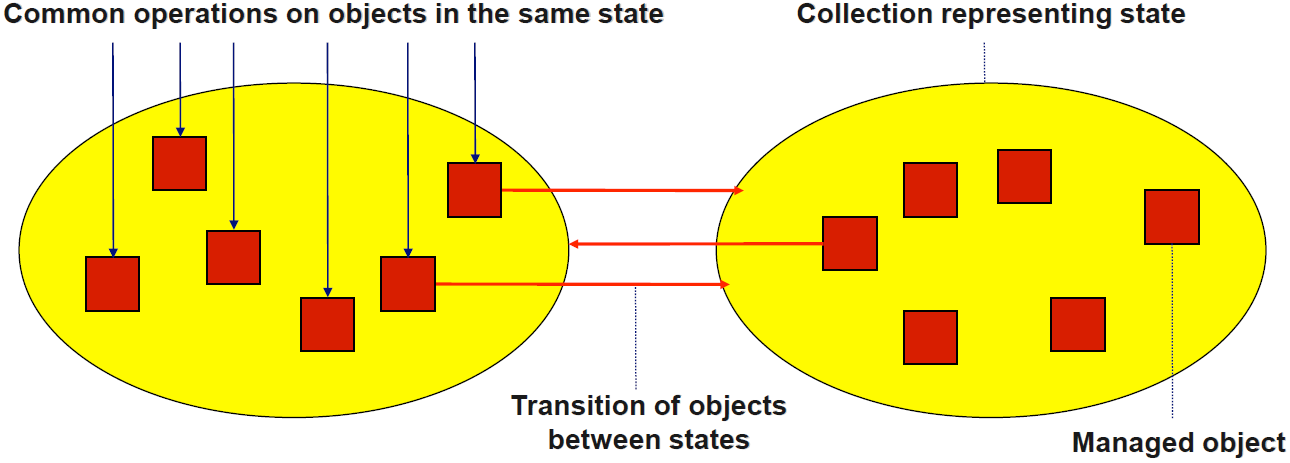
\includegraphics[width=\linewidth]{collection_for_state.png} \\

\textbf{Dynamics}

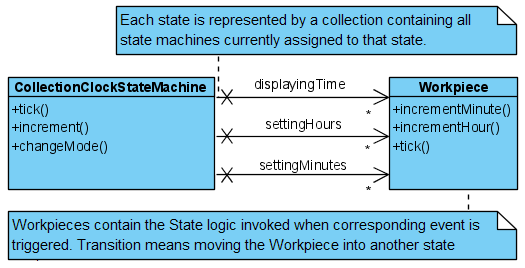
\includegraphics[width=\linewidth]{collection_for_state_dynamic.png}

\subsubsection{Solution}

Jeder Zustand wird von einer Collection repräsentiert, die alle State Machines enthaltet

\subsubsection{Consequences}
\textbf{Benefits}
\begin{itemize}
    \item Nicht notwendig eine Klasse per State zu erstellen
    \item Optimiert für mehrere Objekte (State Machines) in einem bestimmten Zustand
    \item Objekt Collection bestimmt implizit dessen Zustand $\rightarrow$ Der Zustand muss nicht intern repräsentiert werden
    \item Kann mit anderen State Machine (Objects / Methods) Ansätzen kombiniert werden
\end{itemize}
\vspace{10pt}
\textbf{Liabilities}
\begin{itemize}
    \item Kann zu einem komplexeren State Manager führen
\end{itemize}

